\begin{textarea}[]
  \only<1>{
    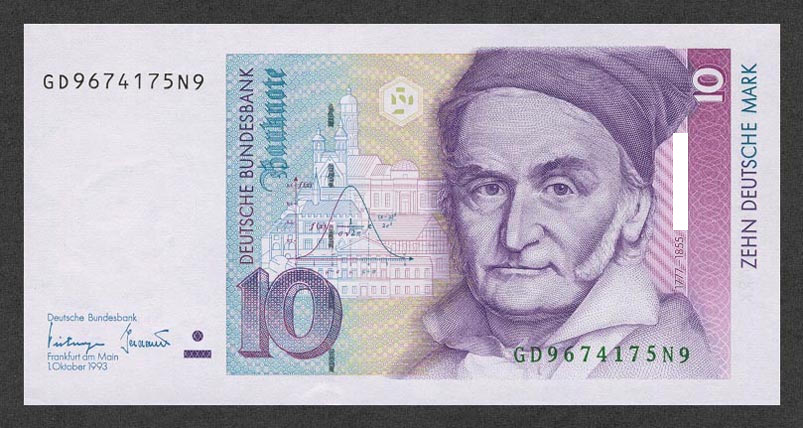
\includegraphics[height=0.5\linewidth]{categories/media/vips/10_DM_Serie4_Vorderseite}
  }
  \only<2>{
    Who is Carl Friedrich Gau{\ss}?
  }
\end{textarea}

\begin{textarea}[]
  \only<1>{
    \begin{columns}[c]
      \column{.5\textwidth}
        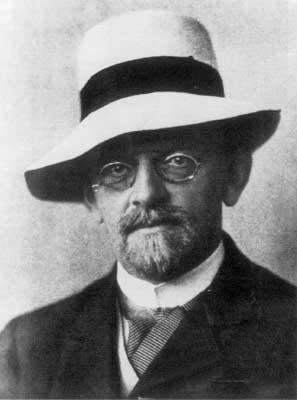
\includegraphics[height=0.5\linewidth]{categories/media/vips/Hilbert}
      \column{.5\textwidth}
       This German mathematician is said to be one of the most influential ones, even though he left us with $23$ unsolved problems.
    \end{columns}
  }
  \only<2>{
    Who is David Hilbert?
  }
\end{textarea}

\begin{textarea}[]
  \only<1>{
    \begin{columns}[c]
      \column{.5\textwidth}
      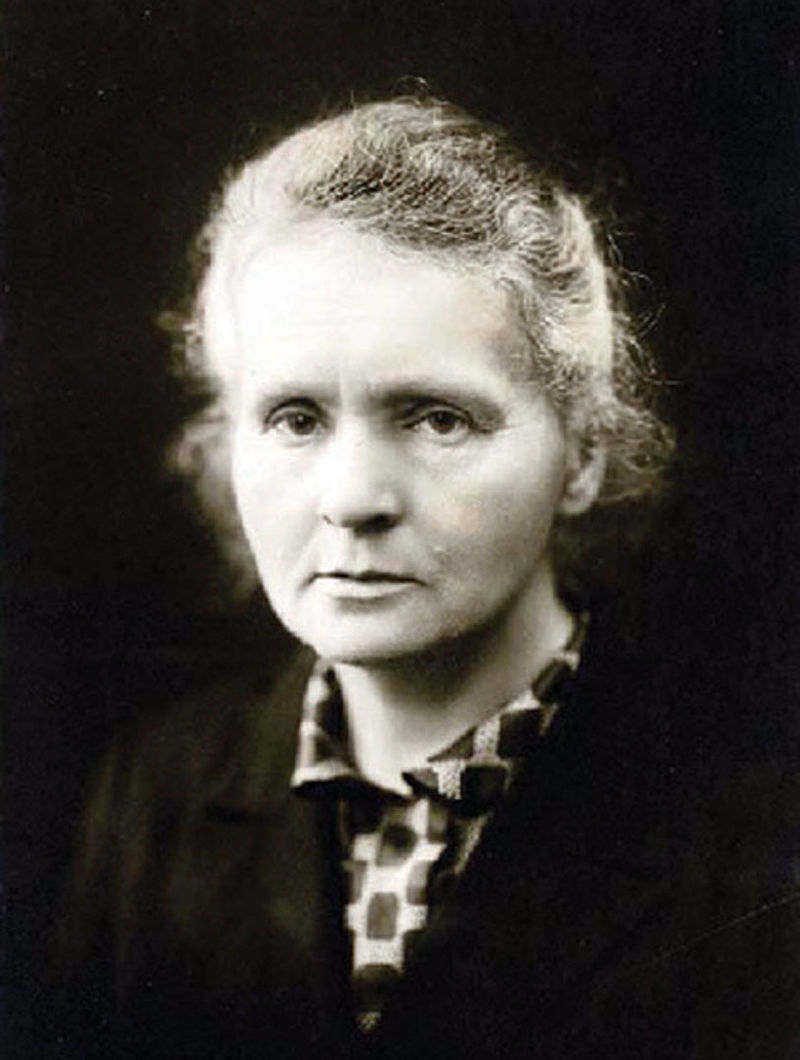
\includegraphics[height=1.0\linewidth]{categories/media/vips/MarieCurie}
      \column{.5\textwidth}
      This Polish scientist was the first to be rewarded with a Nobel prize.
    \end{columns}
  }
  \only<2>{
    Who is Marie Curie?
  }
\end{textarea}

\begin{textarea}[]
  \only<1>{
  	 \begin{columns}[c]
  	 	\column{.5\textwidth}
    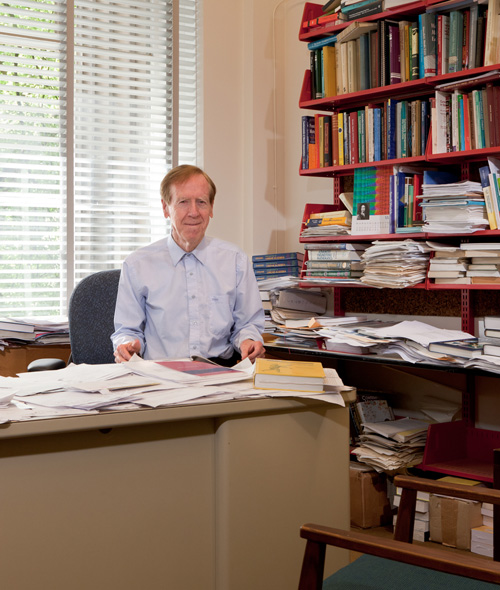
\includegraphics[height=1\linewidth]{categories/media/vips/Strang8}
  	 	\column{.5\textwidth}
  	 	Famous for his research, but also for his presentation style in lectures on MIT Open Course Ware. 
  	 	
  	 	He was here once.
  	 \end{columns}

  
  }
  \only<2>{
    Who is Gilbert Strang?
  }
\end{textarea}





\begin{textarea}[]
  \only<1>{
    With her landmark contributions to abstract algebra, she was the first woman who habilitated in mathematics.
  }
  \only<2>{
    Who is Emmy Noether?
  }
\end{textarea}
